\documentclass{article}
\usepackage{graphicx}
\title{Rebuttal}
\author{Shrinath Deshpande, Anurag Purwar}

\begin{document}
\maketitle
We are grateful to all of the reviewers, who took out their valuable time to review our paper. This work would be incomplete without the reviewers' inputs.
The reviewers' comments are given in \emph{italicized}, whereas our answers are in normal text.

\section{Reviewer 1}
%The authors propose applying machine learning techniques to solving planar four-bar linkage problems. The authors claim gaps exist in existing methods that do not account for circuit and branch defects in the synthesis process.
%Significant technical deficiencies and several editorial issues exist in the submitted manuscript. Therefore, this reviewer must recommend a reject and encourage the authors to make major revisions before the manuscript could be acceptable for publication.
\begin{itemize}
  \item \emph{
Overall, the paper lacks a clear motivation for why the described method is required.
The authors highlight several gaps in existing methods identified by the literature.
However, the authors do not explain how those defects affect current practice or why a new method is necessary.
While gaps may exist in current methods, are those gaps significant enough to not produce accurate results? If so, why? The introduction of the manuscript reads as a background knowledge section.
This reviewer recommends the authors include a new introduction that strongly motivates their work described in the manuscript and rename the current introduction.
Example questions for identifying a motivation are: what stakeholders benefit from the authors' contributions? What are the expected benefits and/or impacts of the novel contributions? To what type of real, practical problems does the method apply?
Overall, the paper lacks a clear motivation for why the described method is required.
Absent a strong motivation, the manuscript reads as if the authors pursued a machine-learning problem for the sake of machine learning. This reviewer finds little value in answering these types of research questions.
Manuscript lacks a clear motivation linked to the practitioner.
The research objective, methods, and approach are not clear.
}

Thank you for pointing out an important point.
We have rewritten the introduction section to clearly explain motivation and overview of the approach.
The motivation subsection clearly explains the significance of the gaps in current practices.
We summarize the motivation as follows,

The classical mechanism synthesis problem deals with computing type and dimensions of a linkage system for performing specific tasks, which are categorized as the path, motion and function generation.
Path generation task aims to synthesize a mechanism which can guide a point along a prescribed path.
On the other hand, the objective of motion generation task is to synthesize a mechanism which can guide a rigid body along a prescribed motion.
The prescribed path is a time sequence of positions, whereas the prescribed motion is a time sequence of positions and orientations.

The majority of mechanism synthesis methods are based on the precision point approach.
This approach is a clever approximation trick to solve the synthesis tasks, where the task is discretized into precision points.
These points instead of the actual task, are treated as interpolation or approximation task for mechanism synthesis.
However, this way of formulation loses important information about the actual continuous task and can lead to solutions with the order, circuit and branch defects.
The defect in a mechanism renders itself useless for its intended application.

\begin{figure}
\centering
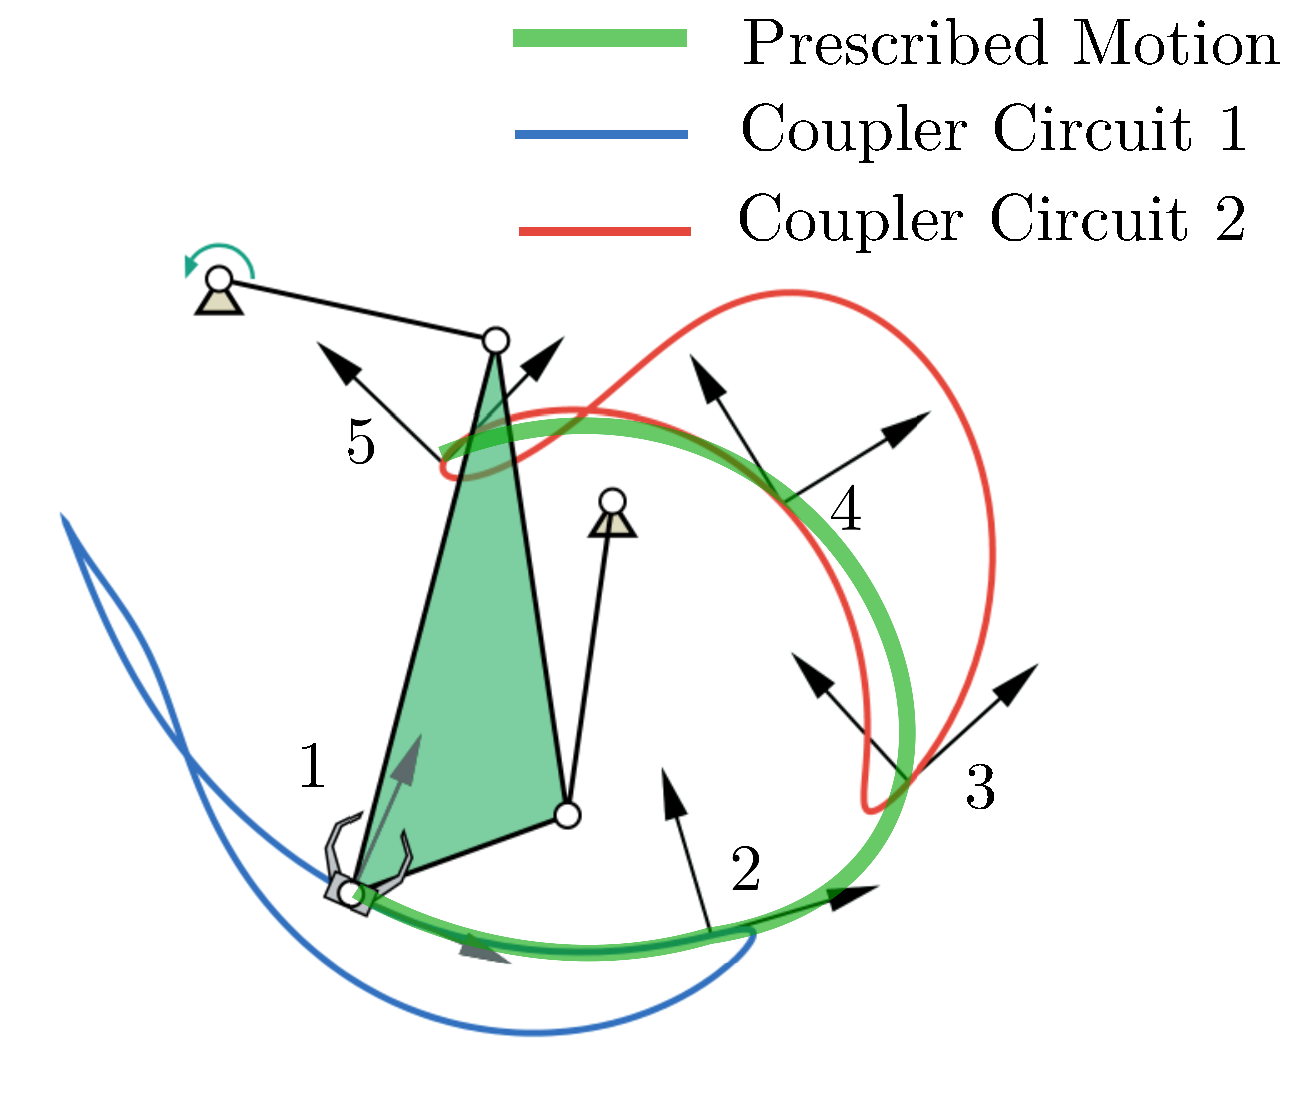
\includegraphics[width=200pt]{fig_circuit_defect.eps}
  \caption{The mechanism synthesis problem for the prescribed motion.
  The four-bar mechanism obtained using the precision position approach suffers from circuit defect, as no coupler circuit passes through all precision positions.}
\label{circuit_defect}
\end{figure}

Figure~\ref{circuit_defect} shows the prescribed motion and its discretized precision positions.
In the case of motion generation problem, a four-bar can go through at most five precision positions and it is called as classical Burmester~\cite{Burmester86} problem.
For this type of problem, only finite solutions exist and in this case only one solution is obtained as shown in the Fig.~\ref{circuit_defect}.
Although it can be seen that coupler of the four-bar passes exactly through five precision positions, it can not do it without changing the circuit.
A circuit represents an assembly mode in which the mechanism is put together.
This phenomenon is called circuit defect in the linkage, which makes the linkage useless for the prescribed task.
Even if the defect-free solution is found, the coupler motion in-between the precision points may go through undesired position and orientation.
This happens because the method discards the functional aspect of continuous motion and turns it into a vacuous interpolation problem.
This tells us that just finding a defect-free linkage with respect to the precision positions is not enough to qualify as a useful mechanism.

To capture the complete prescribed task, we represent it as a continuous parametric curve.
The objective is to find a linkage, that has a coupler motion or path compatible with the task.
Next step is to conduct a search in the space of linkage parameters to find linkages with coupler motions compatible with the prescribed task.
Although global search methods can be applied for finding solutions, we employ an efficiently clustered database and Powell's local search method to come up with a variety of different solutions.
We exploit machine learning to maximize the diversity, and for efficient storage of the linkage database.
The outcomes of this approach are a large number of diverse concept solutions.
The importance of diverse concept generation is mentioned in motivation subsection by following lines,
``Thus, the synthesis method should be prolific in terms of concept generation to 1) realize the potential of attainable design possibilities, and 2) have the agility to adapt a design to evolving requirements."
\\

  \item \emph{
Further, most of the citations in the manuscript, not including the authors' previous work, are over 10 years old.
}

Thanks, we have added recent citations reporting the work in the area of mechanism synthesis and machine learning applications to mechanisms.
\\

  \item \emph{
Instead, the authors should motivate their work with important use cases that address necessary research questions for an identified stakeholder. Tell the reader why this work is important? The authors claim the current approaches are useless for practical applications. What are the practical applications and what are their requirements? The authors do include two use cases, but their practical relevance is not discussed.
}

Thank you for your comments.
We have added the example shown in the Fig.~\ref{circuit_defect} to the motivation section, which clearly explains the limitations of current practices.
We have used the same example in the example section to clearly juxtapose our results against results of precision point approach.
\\

  \item \emph{
 The reason for employing machine learning techniques is artificially explained in one sentence at the end of Section 3.3. Expand the reason for employing machine learning.
}

We have expanded the reason for employing machine learning techniques in the subsection titled 'Dimensionality Reduction using Auto-Encoders' as follows,

``In order to have efficient query operations, we perform Hierarchical Clustering; a method that summarizes and creates a hierarchy in the database.
Clustering in higher dimensions suffers from \emph{Curse of Dimensionality}\cite{marimont1979}, thus we first perform dimensionality reduction using Auto-encoder Neural Networks.
Auto-encoder is a powerful mapping model, which learns to encode the input data in very compact representation and can reconstruct the input with minimal error; performing much better than Principal Component Analysis\cite{hinton2006}.
This nonlinear mapping by auto-encoder can greatly improve the representation of data for clustering~\cite{song2013}."

In addition to that, we have added following lines to explain the motivation behind using clustering,
``We use machine learning techniques such as clustering and data-compression using auto-encoder neural networks to come up with good initial guesses for local optimization.
First, We cluster the database using hierarchical clustering algorithm.
Then, we find representative data point in each cluster called cluster center and form their set.
This set of cluster centers represent a diverse group of linkages.
When a query is raised in the database, the first step is to search for neighbors in the set of cluster centers.
This often yields a diverse set of neighbors and is used as a set of initial guesses for local optimization.
"
\\

  \item \emph{
  In Fig. 1 (overview), should an arrow return from ``Local Optimizer" to ``Accurate?" or is the assumption that all outputs from the ``Local Optimizer" are accurate?
}

Thank you for mentioning that.
We have fixed it.
\\

  \item \emph{
The values used in the sensitivity analysis are not justified. How did the authors choose the values?
}

Thank you for the comment. We have added following line,
``The link ratios are chosen such that, small changes in some parameters lead to a topological change in the coupler curve."
\\

  \item \emph{
The quality of research methods cannot be assessed.
}

We have employed already proven techniques such as b-spline interpolation, hierarchical clustering, data compression using auto-encoders, Powell's local search.
We have formulated the signatures of coupler path and motion, based on proven 2D curve matching technique by Cui et al.\cite{cui2009}.
We have presented the validation of the partial matching algorithms using examples in section 4.
Finally, we present two case studies, where we obtain the diverse set of useful linkage solutions for path and motion generation problem.
\\

  \item \emph{
The conclusion is too short. It lacks a critical discussion of the research. The authors should critically assess the proposed approach.
}

Thanks for the important feedback, we have modified the conclusion by adding critical assessment of the approach as follows,
`` The problem formulation is invariant with respect to translation, orientation, and scaling.
Hence, constraints like geometric restrictions on pivots have to be addressed after finding feasible solutions for the task.
The approach is general enough to be extended to higher order linkage systems for which there are even fewer methods available for synthesizing defect-free solutions.
However, the database size increases exponentially with the number of links in the mechanisms.
As an example, a Watt type six-bar database needs to be roughly 400 times larger than four-bar database.

A potential solution to this problem could be to use learning based methods, where the pattern is learned instead of storing all of the information.
Overall, the method provides a holistic approach towards the prescribed path and motion synthesis and encourages artificial intelligence techniques to make an impact.
"

  \item \emph{
 Review the usage of ``that" versus ``which". There are some instances where the usage should be reversed.
 \\
 Several instances exist throughout the manuscript where nouns could benefit from having a ``the" put in from of them. For example, the first sentence of Section 5.1 reads as, ``Each data point in the database consists of discrete..." Instead, the sentence should read as, ``Each data point in [the] database consists of discrete..."
 Check usage of hyphens. Inconsistent usage exists in the manuscript.
 }

 Thanks for the comments. We have revised the text and fixed it.
\\

\end{itemize}

\section{Reviewer 2}

\begin{itemize}
  \item \emph{
$1$. Please provide brief descriptions (possibly with examples) of circuit and branch defects that
occur when using existing synthesis methods.
}

Thanks for raising this point.
We have added one example in the introduction section, to illustrate the defects in mechanisms when using existing synthesis methods.
\\

  \item \emph{
  $2$. In Figure 2b, why is the range of parameter $t$ for $\theta(t)$ is only 0-50, rather than 0-100?
}

Thank you for the comment. It was a plotting mistake. We have fixed it.
\\

  \item \emph{
$3.$ In Algorithm 2, Line 8, should it be $\theta(tmp)$ instead of $\kappa(tmp)$ ?\\
$4.$ Please check the parenthesis in Equation 5.\\
$6.$ There are several typos involving subscripts all throughput the paper. Please fix them.
}

Thanks for the comments. We have fixed them.
\\

  \item \emph{
$5.$ In Figure 15, $X$ and $\tilde{X}$ mismatch the input and output vectors shown in the diagram.
}

Figure 15 shows $X$ as the input and $\tilde{X}$ as the output of auto-encoder network, which matches with the description.
The query regarding the mismatch is not clear to us.
Could you please elaborate on the query?
\\


  \item \emph{
$7.$ In section 5.1, it is argued that Euclidean distance is used as the distance metric in latent space for
computational efficiency, whereas in section 6.1, $(1 − Cn)$ is mentioned as the distance
metric. Please clarify.
}

Thanks for the feedback. We have made changes in the text to clarify which metric is used at what point.
In section 5.1, we added following lines, ``The distance metric used for clustering is the Euclidean distance in the latent space.
Although the more accurate distance metric is distance function discussed in sec 3, it is very expensive to calculate it for the entire database.
Signatures with ${O}(m)$ points take ${O}(m\log{}m)$ time for each comparison and there are ${O}(N^2)$ number of comparisons to be made for the database of $N$ points.

Now, when the user raises a query, we use the distance function from sec.3 for finding $k$ nearest neighbors among $1500$ cluster centers.
If a cluster center is not sufficiently close, we descend into its corresponding cluster to find the closest data point.
The distance metric for finding neighbors among cluster centers is $1-Cn_{max}$ in Eq. 5.  "
\\

  \item \emph{
$8.$ It is unclear how local optimization is performed after finding the nearest cluster centers. Is the
search performed in each cluster independently? Are multiple paths/motions in the database
combined with partial matching? Please elaborate.
}

Thanks for the comments.
We use the cluster centers as independent initial guesses and do a local search on each initial guess independently.
We have added following lines in section 5 to clarify that.

``When a query is raised in the database, the first step is to search for neighbors in the set of cluster centers.
This often yields a diverse set of neighbors, and is used as a set of independent initial guesses for local optimization."
\\


  \item \emph{
$9.$ Please comment on how this approach can be extended to handle process specific constraints?
For example, the pivots should lie above ground in show-shoveling case study (6.2).
}

Thank you for mentioning that. We have added following lines in the conclusion.
``The partial matching metric although more accurate, but is expensive in terms of computation cost.
Thus, we use Euclidean metric in the latent space of compressed data for hierarchical clustering.
The formulation is invariant with respect to translation, orientation, and scaling.
Hence, constraints like geometric restrictions on pivots, have to be addressed after finding feasible solutions for the task."

\end{itemize}

\bibliographystyle{purwar}
\bibliography{References}

\end{document}

